	\documentclass[10pt,oneside]{CBFT_book}
	% Algunos paquetes
	\usepackage{amssymb}
	\usepackage{amsmath}
	\usepackage{graphicx}
	\usepackage{libertine}
	\usepackage[bold-style=TeX]{unicode-math}
	\usepackage{lipsum}

	\usepackage{natbib}
	\setcitestyle{square}

	\usepackage{polyglossia}
	\setdefaultlanguage{spanish}
	



	\usepackage{CBFT.estilo} % Cargo la hoja de estilo

	% Tipografías
	% \setromanfont[Mapping=tex-text]{Linux Libertine O}
	% \setsansfont[Mapping=tex-text]{DejaVu Sans}
	% \setmonofont[Mapping=tex-text]{DejaVu Sans Mono}

	%===================================================================
	%	DOCUMENTO PROPIAMENTE DICHO
	%===================================================================

\begin{document}

% =================================================================================================
\chapter{Introducción a la mecánica cuántica relativista}
% =================================================================================================

Consideremos una partícula libre por el momento 
\[
	H =
\]
\[
	P_\mu = i \hbar \partial_\mu = 
\]
\[
	fiesta
\]
\[
	fiesta
\]
\[
	i \hbar \dpar{\psi}{t} = - \frac{\hbar^2}{2m} \nabla^2 \psi
\]
\[
	cuenta 
\]
\[
	resultqado
\]
\[
	d
\]
\[
	conti
\]
que es una analogía de la conservación de la carga en electrodinámica.
Tenemos entonces una especie de conservación de la probabilidad. Note que 
\[
	a
\]
\[
	E
\]

Pero esto se ponde muy complicado debido a la raíz

\subsection{La ecuación de Klein-Gordon}

Conserva el cuadrado para no complicar demasiado los reemplazos. Entonces 
\[
	H^2 = E^2 = 
\]
\[
	-
\]
\[
	p
\]
\[
	a
\]
\[
	s
\]
\[
	res
\]

El problema es que no puede asegurarse que esta $\rho$ sea definida positiva, lo cual sería necesario para 
seguir una coherencia.

\[
	a
\]
\[
	a
\]
\[
	a
\]
\[
	a
\]
Necesito considerar $E<0$ pues $E=\pm\sqrt{c^2p^2+m^2c^4}$ y la base debe ser completa.

Es positiva si tuviese $E<0$ pero esto causa el problema de tener materia inestable, pues nunca se alcanza el 
fundamental. Acá muere en este atolladero la ecuación de Klein-Gordon.

\subsection{La ecuación de Dirac}

Dirac parte de pedir una ecuación lineal en el impulso \vb{p}
\[
	H
\]
con $\beta,\vb{\alpha},\vb{p}$ operadores.
\[
	H^2
\]
\[
	H^2
\]
\[
	H^2
\]
\[
	H^2
\]
Como se ve, estos no pueden ser simples escalares. Dirac pide 
\begin{itemize}
 \item $\vb{\alpha},\beta$ hermíticos
 \item $\beta^2=1 \; \alpha^2=1$ autovalores $\pm 1$
 \item traza nula
 \[
	a
 \]
 \item dimensión par 
 \[
	a
 \]
\end{itemize}

\[
	a
\]
\[
	a
\]
\[
	a
\]
\[
	a
\]

Ahora tenemos una densidad de proababilidad como requiere la naturaleza.

\subsection{Ejemplo: partícula libre quieta}

Sea una partícula libre en reposo,
\[
	\vb{p} = 0 \qquad H=\beta m c^2
\]
\[
	i \hbar \dpar{\psi}{t} = \beta m c^2 \psi
\]
\[
	i
\]
Tenemos cuatro ecuaciones, dos con energía positiva y dos con energía negativa
\[
	a
\]
Como aún tenemos degeneración de orden dos, necesitaremos un operadore que conmute con el $H$
\[
	a
\]
\[
	b
\]
Podemos identificar 
\[
	S
\]
\[
	p \neq = 0  \Rightarrow [H, vb{\Sigma}] = 2ic \vb{\alpha} \times \vb{p}
\]

\subsection{Energías negativas}

Como $E = \pm  \sqrt{ c^2 p^2 + m^2 c^4 } $ hay $E<0$ y además un {\it gap} de ancho $2mc^2$ entre ellas.
Las $E<0$ harían que la materia jamás alcance un estado fundamental y por ende jamás se estabilice.
Dirac piensa que los estados de $E<0$ están todos llenos. No decaen más electrones allí dentro. Es el mar de 
Dirac. Iluminando ese vacío se lo puede excitar.

\begin{figure}[htb]
	\begin{center}
	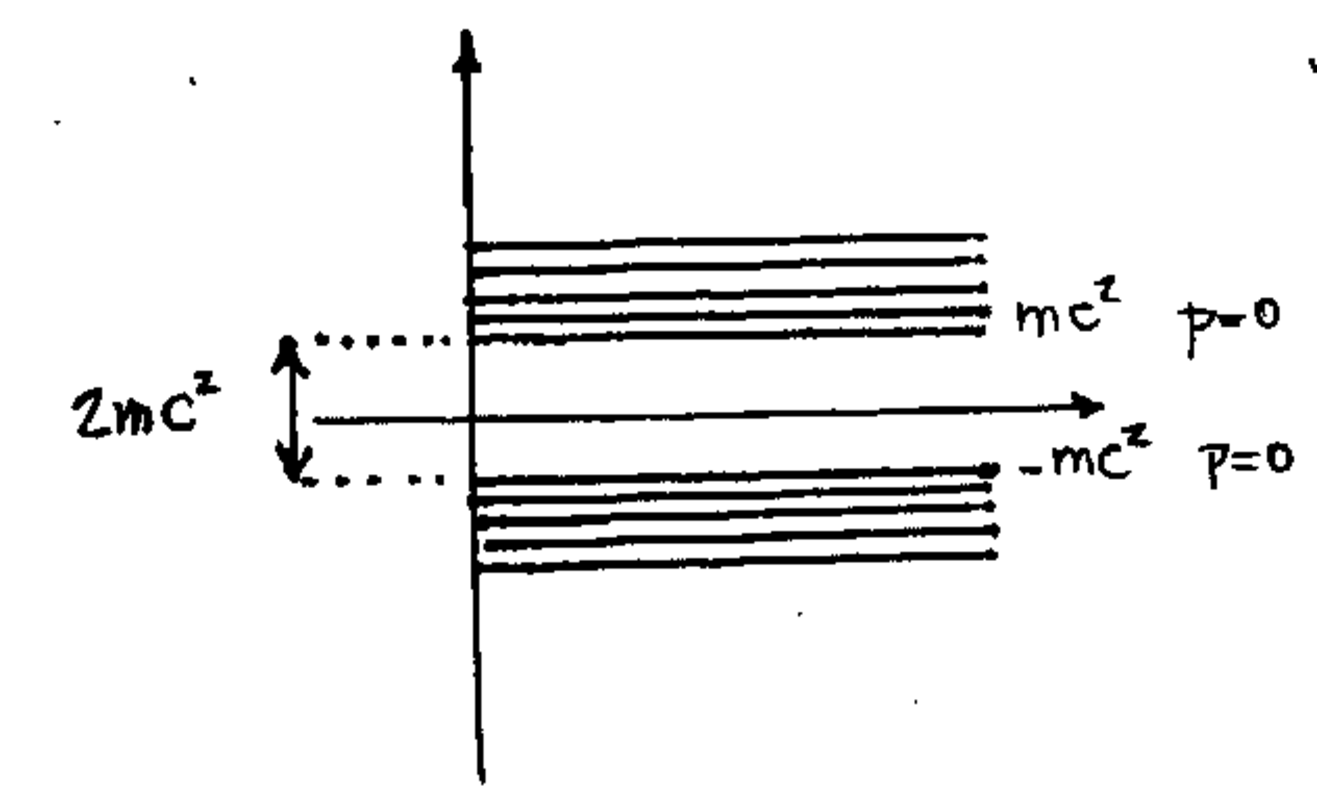
\includegraphics[width=0.6\textwidth]{images/teo2_13.pdf}
	\end{center}
	\caption{}
\end{figure} 

Podemos hacer saltar a la zona positiva una carga $(-e)$ dejando un huevo positivo (equivalente a una carga 
$+e$). Es una creación e pares $\gamma \to e^-e^+$, sin embargo el proceso inverso $ e^-e^+ \to \gamma$ de 
aniquilación de pares ocurre prontamente.
Se observó experimentalmente.

\begin{figure}[htb]
	\begin{center}
	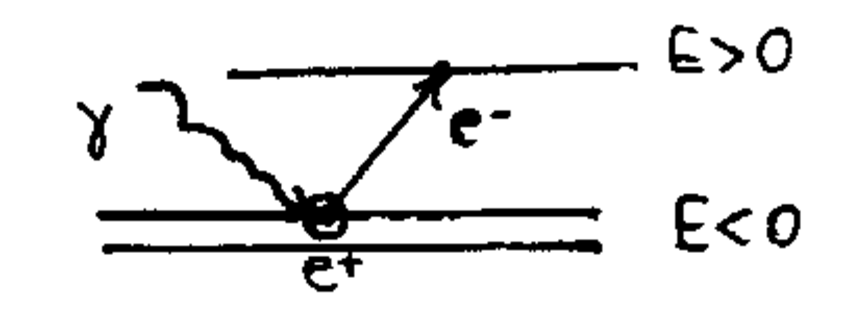
\includegraphics[width=0.6\textwidth]{images/teo2_14.pdf}
	\end{center}
	\caption{}
\end{figure} 


% \bibliographystyle{CBFT-apa-good}	% (uses file "apa-good.bst")
% \bibliography{CBFT.Referencias} % La base de datos bibliográfica

\end{document}
